\section{Introduction}
\label{sec:introduction}

A useful historical answer needs the right period.
Consider a question about a radio programme's hosts between 1977 and 1995.
Several successive hosts belong in the answer.
Keeping only the latest host loses part of that history.
Likewise, a stadium can host two teams during overlapping periods.
A newer team does not automatically replace an older tenant.
Both examples occur in the natural passages of TimeQA~\citep{chen2021timeqa}.

Retrieval-augmented generation must fit this evidence into a limited context~\citep{lewis2020rag}.
Text relevance identifies the topic.
Temporal selection determines which descriptions can support the requested period.
That selection becomes harder when sources give coarse dates.
An appointment reported as occurring in a year does not identify its exact day.
A later record can establish a possible replacement without establishing when it happened.
Committing to an arbitrary date hides this distinction from the reader.

\begin{figure*}[t]
\centering
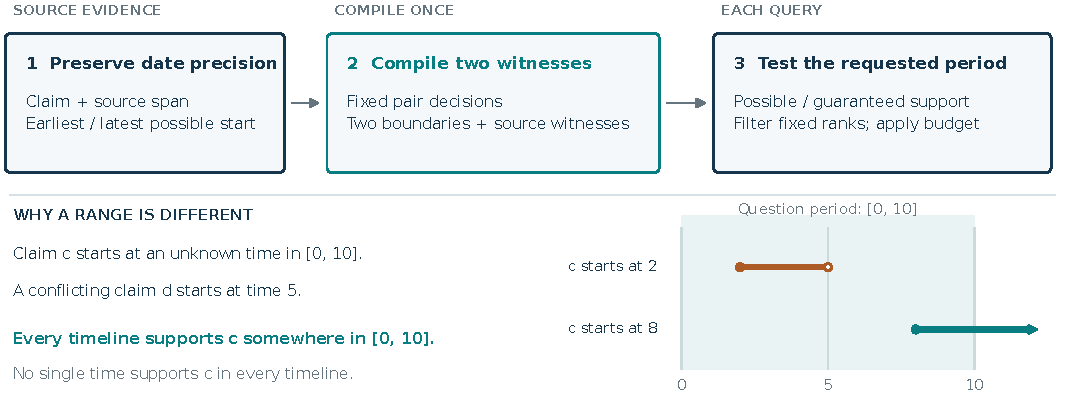
\includegraphics[width=\textwidth]{figures/architecture.pdf}
\caption{The compiler preserves uncertain occurrence dates and records two direct replacement witnesses per claim. Query-time tests return possible and guaranteed support for the requested period. The lower panel illustrates two allowed timelines. Claim $c$ has support somewhere in $[0,10]$ in every timeline, although no single time guarantees support. The times are illustrative units.}
\label{fig:architecture}
\end{figure*}

Existing temporal memories already preserve fact histories and invalidate earlier claims.
Graphiti applies direct contradiction decisions~\citep{rasmussen2025zep,graphiti2026source}.
NuggetIndex combines source spans, validity intervals, and lifecycle states~\citep{zerhoudi2026nuggetindex}.
DeFuzzRAG and IA-RAG handle fuzzy dates and interval-based retrieval~\citep{chen2026defuzzrag,wang2026iarag}.
These mechanisms make date interpretation central to evidence selection.
We study the exact decisions available before choosing one interpretation of an uncertain occurrence date.

Our central question is simple:
\emph{Which claims can be removed without discarding support under an allowed timeline?}
We also ask which claims have support under every allowed timeline.
These questions produce two useful sets.
\emph{Possible support} retains evidence that could apply somewhere in the requested period.
\emph{Guaranteed support} retains evidence that applies somewhere in that period under every permitted date assignment.
Claims with possible but unguaranteed support have unresolved temporal status.

The second set requires care.
Suppose a claim begins sometime between times 0 and 10.
A conflicting claim begins at time 5.
If the first claim begins earlier, it contributes before the replacement.
If it begins later, it contributes from its own start.
Every allowed timeline therefore supports it somewhere in $[0,10]$.
Yet there is no single time when all timelines support it.
Intersecting the query with a certainly active interval would miss this evidence.
Figure~\ref{fig:architecture} illustrates the distinction.

We derive a compact solution for a fixed direct replacement policy.
Each claim has an earliest and latest possible start.
One witness determines when replacement becomes unavoidable.
A second witness determines when replacement becomes possible.
These two witnesses answer every point and period query without enumerating timelines.
They expose which source decisions caused an exclusion.

Our contribution has three parts.
First, we give exact support tests and prove that two witnesses suffice.
Two are necessary in the worst case among direct witness subsets.
Second, we prove refinement and error-locality properties.
We also certify exactly when every timeline returns the same ranked claim context.
More precise dates narrow possible support and expand guaranteed support.
Changing one directed replacement decision affects only its target claim.
Third, we establish a source-grounded evaluation protocol that preserves complete answer sets and original passage text.
It separates executor correctness, yearly snapshot selection, and natural-passage retrieval.

This protocol reveals why temporal metrics need the full requested scope.
In TempLAMA, a changed first answer often remains valid in the new annual answer set.
In TimeQA, a range can include successive answers, concurrent answers, or several names for one answer.
The compiler addresses uncertainty in occurrence dates.
The evaluation measures how temporal selection interacts with the evidence that a question requests.
